% ******************************* PhD Thesis Template **************************
% Please have a look at the README.md file for info on how to use the template

% \documentclass[a4paper,12pt,default,print,index,authoryear]{classes/PhDThesisPSnPDF} %final version
% \documentclass[a4paper,12pt,times,chapter,index,authoryear]{classes/PhDThesisPSnPDF} % chapter mode
\documentclass[a4paper,12pt,default,draft,index,authoryear]{classes/PhDThesisPSnPDF} % draft mode


% ******************************************************************************
% ******************************* Class Options ********************************
% *********************** See README for more details **************************
% ******************************************************************************

% `a4paper'(The University of Cambridge PhD thesis guidelines recommends a page
% size a4 - default option) or `a5paper': A5 Paper size is also allowed as per
% the Cambridge University Engineering Deparment guidelines for PhD thesis
%
% `11pt' or `12pt'(default): Font Size 10pt is NOT recommended by the University
% guidelines
%
% `oneside' or `twoside'(default): Printing double side (twoside) or single
% side.
%
% `print': Use `print' for print version with appropriate margins and page
% layout. Leaving the options field blank will activate Online version.
%
% `index': For index at the end of the thesis
%
% `draftclassic': For draft mode without loading any images (same as draft in book)
%
% `draft': Special draft mode with line numbers, images, and water mark with
% timestamp and custom text. Position of the text can also be modified.
%
% `abstract': To generate only the title page and abstract page with
% dissertation title and name, to submit to the Student Registry
%
% `chapter`: This option enables only the specified chapter and it's references
%  Useful for review and corrections.
%
% ************************* Custom Page Margins ********************************
%
% `custommargin`: Use `custommargin' in options to activate custom page margins,
% which can be defined in the preamble.tex. Custom margin will override
% print/online margin setup.
%
% *********************** Choosing the Fonts in Class Options ******************
%
% `times' : Times font with math support. (The Cambridge University guidelines
% recommend using times)
%
% `fourier': Utopia Font with Fourier Math font (Font has to be installed)
%            It's a free font.
%
% `customfont': Use `customfont' option in the document class and load the
% package in the preamble.tex
%
% default or leave empty: `Latin Modern' font will be loaded.
%
% ********************** Choosing the Bibliography style ***********************
%
% `authoryear': For author-year citation eg., Krishna (2013)
%
% `numbered': (Default Option) For numbered and sorted citation e.g., [1,5,2]
%
% `custombib': Define your own bibliography style in the `preamble.tex' file.
%              `\RequirePackage[square, sort, numbers, authoryear]{natbib}'.
%              This can be also used to load biblatex instead of natbib
%              (See Preamble)
%
% **************************** Choosing the Page Style *************************
%
% `default (leave empty)': For Page Numbers in Header (Left Even, Right Odd) and
% Chapter Name in Header (Right Even) and Section Name (Left Odd). Blank Footer.
%
% `PageStyleI': Chapter Name next & Page Number on Even Side (Left Even).
% Section Name & Page Number in Header on Odd Side (Right Odd). Footer is empty.
%
% `PageStyleII': Chapter Name on Even Side (Left Even) in Header. Section Number
% and Section Name in Header on Odd Side (Right Odd). Page numbering in footer

% Uncomment to change page style
\pagestyle{PageStyleII}

% ********************************** Preamble **********************************
% Preamble: Contains packages and user-defined commands and settings
% ******************************************************************************
% ****************************** Custom Margin *********************************

% Add `custommargin' in the document class options to use this section
% Set {innerside margin / outerside margin / topmargin / bottom margin}  and
% other page dimensions
\ifsetCustomMargin
  \RequirePackage[left=37mm,right=30mm,top=35mm,bottom=30mm]{geometry}
  \setFancyHdr % To apply fancy header after geometry package is loaded
\fi

% Add spaces between paragraphs
%\setlength{\parskip}{0.5em}
% Ragged bottom avoids extra whitespaces between paragraphs
\raggedbottom
% To remove the excess top spacing for enumeration, list and description
%\usepackage{enumitem}
%\setlist[enumerate,itemize,description]{topsep=0em}

% *****************************************************************************
% ******************* Fonts (like different typewriter fonts etc.)*************

% Add `customfont' in the document class option to use this section

\ifsetCustomFont
  % Set your custom font here and use `customfont' in options. Leave empty to
  % load computer modern font (default LaTeX font).
  %\RequirePackage{helvet}

  % For use with XeLaTeX
  %  \setmainfont[
  %    Path              = ./libertine/opentype/,
  %    Extension         = .otf,
  %    UprightFont = LinLibertine_R,
  %    BoldFont = LinLibertine_RZ, % Linux Libertine O Regular Semibold
  %    ItalicFont = LinLibertine_RI,
  %    BoldItalicFont = LinLibertine_RZI, % Linux Libertine O Regular Semibold Italic
  %  ]
  %  {libertine}
  %  % load font from system font
  %  \newfontfamily\libertinesystemfont{Linux Libertine O}
\fi

% *****************************************************************************
% **************************** Custom Packages ********************************

% ************************* Algorithms and Pseudocode **************************

%\usepackage{algpseudocode}


% ********************Captions and Hyperreferencing / URL **********************

% Captions: This makes captions of figures use a boldfaced small font.
%\RequirePackage[small,bf]{caption}

\RequirePackage[labelsep=space,tableposition=top]{caption}
\renewcommand{\figurename}{Fig.} %to support older versions of captions.sty


% *************************** Graphics and figures *****************************

%\usepackage{rotating}
%\usepackage{wrapfig}

% Uncomment the following two lines to force Latex to place the figure.
% Use [H] when including graphics. Note 'H' instead of 'h'
%\usepackage{float}
%\restylefloat{figure}

% Subcaption package is also available in the sty folder you can use that by
% uncommenting the following line
% This is for people stuck with older versions of texlive
%\usepackage{sty/caption/subcaption}
\usepackage{subcaption}

% ********************************** Tables ************************************
\usepackage{booktabs} % For professional looking tables
\usepackage{multirow}

%\usepackage{multicol}
%\usepackage{longtable}
%\usepackage{tabularx}


% *********************************** SI Units *********************************
\usepackage{siunitx} % use this package module for SI units


% ******************************* Line Spacing *********************************

% Choose linespacing as appropriate. Default is one-half line spacing as per the
% University guidelines

\doublespacing
% \onehalfspacing
% \singlespacing


% ************************ Formatting / Footnote *******************************

% Don't break enumeration (etc.) across pages in an ugly manner (default 10000)
%\clubpenalty=500
%\widowpenalty=500

%\usepackage[perpage]{footmisc} %Range of footnote options


% *****************************************************************************
% *************************** Bibliography  and References ********************

%\usepackage{cleveref} %Referencing without need to explicitly state fig /table

% Add `custombib' in the document class option to use this section
\ifuseCustomBib
   \RequirePackage[square, sort, numbers, authoryear]{natbib} % CustomBib

% If you would like to use biblatex for your reference management, as opposed to the default `natbibpackage` pass the option `custombib` in the document class. Comment out the previous line to make sure you don't load the natbib package. Uncomment the following lines and specify the location of references.bib file

%\RequirePackage[backend=biber, style=numeric-comp, citestyle=numeric, sorting=nty, natbib=true]{biblatex}
%\bibliography{References/references} %Location of references.bib only for biblatex

\fi

% changes the default name `Bibliography` -> `References'
\renewcommand{\bibname}{References}


% ******************************************************************************
% ************************* User Defined Commands ******************************
% ******************************************************************************

% *********** To change the name of Table of Contents / LOF and LOT ************

%\renewcommand{\contentsname}{My Table of Contents}
%\renewcommand{\listfigurename}{My List of Figures}
%\renewcommand{\listtablename}{My List of Tables}


% ********************** TOC depth and numbering depth *************************

\setcounter{secnumdepth}{2}
\setcounter{tocdepth}{2}


% ******************************* Nomenclature *********************************

% To change the name of the Nomenclature section, uncomment the following line

%\renewcommand{\nomname}{Symbols}


% ********************************* Appendix ***********************************

% The default value of both \appendixtocname and \appendixpagename is `Appendices'. These names can all be changed via:

%\renewcommand{\appendixtocname}{List of appendices}
%\renewcommand{\appendixname}{Appndx}

% *********************** Configure Draft Mode **********************************

% Uncomment to disable figures in `draft'
%\setkeys{Gin}{draft=true}  % set draft to false to enable figures in `draft'

% These options are active only during the draft mode
% Default text is "Draft"
\SetDraftText{Draft}

% Default Watermark location is top. Location (top/bottom)
\SetDraftWMPosition{top}

% Draft Version - default is v1.0
\SetDraftVersion{v1.0}

% Draft Text grayscale value (should be between 0-black and 1-white)
% Default value is 0.75
\SetDraftGrayScale{0.8}


% ******************************** Todo Notes **********************************
%% Uncomment the following lines to have todonotes.

%\ifsetDraft
%	\usepackage[colorinlistoftodos]{todonotes}
%	\newcommand{\mynote}[1]{\todo[author=kks32,size=\small,inline,color=green!40]{#1}}
%\else
%	\newcommand{\mynote}[1]{}
%	\newcommand{\listoftodos}{}
%\fi

% Example todo: \mynote{Hey! I have a note}

% *****************************************************************************
% ******************* Better enumeration my MB*************
\usepackage{enumitem}

% *****************************************************************************
% ******************* Extra Packages *************

\usepackage{lipsum}  % for \lipsum[2-4] will print lorem ipsum paragraph 2 to 4.


\usepackage{xspace}
\newcommand{\MATLAB}{\textsc{Matlab}\xspace}
%It is used \xspace in order to prevent the \MATLAB command from eating spaces after it
% xspace package is used in order to prevent eating spaces after the command \MATLAB

\newcommand{\R}{\textsf{R}\xspace}

%Harvard Style

\usepackage{natbib}
%The natbib package  has  two  basic  citation  commands,
%\citet and \citep for textual and parenthetical citations, respectively.
%https://gking.harvard.edu/files/natnotes2.pdf






% ************************ Thesis Information & Meta-data **********************
% Thesis title and author information, refernce file for biblatex
% ************************ Thesis Information & Meta-data **********************
%% The title of the thesis
% \title{Writing your PhD thesis in \texorpdfstring{\\ \LaTeX2e}{LaTeX2e}}
% \title{Movement Variability in the context of Human-Humanoid Imitation}
% \title{Towards the Analysis of Movement Variability in the context of Human-Humanoid Imitation}
% \title{Towards the Analysis of Movement Variability in the context of Human-Humanoid Imitation} %August2017

% \title{Automatic Analysis of Movement Variability in the Context of Human-Humanoid Imitation} %14December2017
\title{Automatic Analysis of Movement Variability} %14December2017


%\texorpdfstring is used for PDF metadata. Usage:
%\texorpdfstring{LaTeX_Version}{PDF Version (non-latex)} eg.,
%\texorpdfstring{$sigma$}{sigma}

% %% Subtitle (Optional)
% \subtitle{Using the CUED template}

%% The full name of the author
\author{Miguel P Xochicale}

%% Department (eg. Department of Engineering, Maths, Physics)
% \dept{Department of Engineering}
\dept{School of Engineering}

%% University and Crest
\university{University of Birmingham}
% Crest minimum should be 30mm.
\crest{
\includegraphics[width=0.2\textwidth]{BirminghamUniversityCrest}}
%% Use this crest, if you are using the college crest
%% Crest long miminum should be 65mm
%\crest{
\includegraphics[width=0.45\textwidth]{University_Crest_Long}}

%% College shield [optional]
% Crest minimum should be 30mm.
%\collegeshield{
\includegraphics[width=0.2\textwidth]{CollegeShields/Kings}}


%% Supervisor (optional)
%% for multiple supervisors, append each supervisor with the \newline command
%\supervisor{Prof. A.B. Supervisor\newline
%Prof. C.D. Supervisor}

%% Supervisor Role (optional) - Supervisor (default) or advisor
% \supervisorrole{\textbf{Supervisors: }}
%% if no title is desired:
% \supervisorrole{}

%% Supervisor line width: required to align supervisors
%\supervisorlinewidth{0.35\textwidth}

%% Advisor (optional)
%% for multiple advisors, append each advisor with the \newline command
%\advisor{Dr. A. Advisor\newline
%Dr. B. Advisor}

%% Advisor Role (optional) - Advisor (default) or leave empty
% \advisorrole{Advisors: }
%% if no title is required
% \advisorrole{}

%% Advisor line width: required to align supervisors
%\advisorlinewidth{0.25\textwidth}


%% You can redefine the submission text:
% Default as per the University guidelines:
% ``This dissertation is submitted for the degree of''
%\renewcommand{\submissiontext}{change the default text here if needed}

%% Full title of the Degree
\degreetitle{Doctor of Philosophy}

% %% College affiliation (optional)
% \college{King's College}

%% Submission date
% Default is set as {\monthname[\the\month]\space\the\year}
\degreedate{June 2018}

%% Meta information
\subject{LaTeX} \keywords{{LaTeX} {PhD Thesis} {Engineering} {University of
Birmingham}}


% ***************************** Abstract Separate ******************************
% To printout only the titlepage and the abstract with the PhD title and the
% author name for submission to the Student Registry, use the `abstract' option in
% the document class.

\ifdefineAbstract
 \pagestyle{empty}
 \includeonly{declaration/declaration, abstract/abstract}
\fi

% ***************************** Chapter Mode ***********************************
% The chapter mode allows user to only print particular chapters with references
% Title, Contents, Frontmatter are disabled by default
% Useful option to review a particular chapter or to send it to supervisior.
% To use choose `chapter' option in the document class

\ifdefineChapter
 \includeonly{chapter3/chapter3}
\fi

% ******************************** Front Matter ********************************
\begin{document}

\frontmatter

\maketitle

% ************************** Thesis Abstract *****************************
% Use `abstract' as an option in the document class to print only the titlepage and the abstract.
\begin{abstract}


% I follow the guidelines of the nature's template for abstracts (https://twitter.com/trevorabranch/status/620699527486373888?lang=en)

%%%%%%%%%%%%%%%%%%%%%%%%%%%%%%%%%%%%%%%%%%%%%%%%%%%%%%%%%%%%%%%%%%%%%%%%%%%%%%%%
%%%%% One or two sentences proving a basic introduction to the field,
%%%%% comprehensible to a scientist in any discipline.
Movement variability is defined as the variations that occur in motor
performance across multiple repetitions of a task and such behaviour is an
inherent feature within and between each persons' movement.
In the previous four decades, research on measurement and understanding of
movement variability with methodologies of nonlinear dynamics has been well established
in areas such as biomechanics, sport science, psychology, cognitive science,
neuroscience and robotics.
%%%%%%%%%%%%%%%%%%%%%%%%%%%%%%%%%%%%%%%%%%%%%%%%%%%%%%%%%%%%%%%%%%%%%%%%%%%%%%%%
%%%%% Two to three sentences of more detailed background,
%%%%% comprehensible to scientist in related disciplines.
Given that traditional methods in time-domain and frequency domain fail to
detect tiny modulations in frequency or phase of time series,
we consider a methodology from nonlinear dynamics called uniform reconstructed state space 
to quantify movement variability which essentially the dynamics of
an unknown system can be reconstructed using one dimensional time series.
As pointed out by Bradley et al. uniform reconstructed state space,
if done right, can guarantee to be topologically identical to the true dynamics
and determine dynamics invariants such as fractal dimension, Kolmogorov-Sinai
entropy or Lyaponov exponents.
These algorithms, however, require time series measured with costly sensors
that provide well sampled data with little noise.
Such requirement is generally a common problem when doing precise
characterisation of time series using dynamic invariants,
to which Bradley et al. proposed additional tools of
nonlinear time series analysis for practitioners such as surrogate data,
permutation entropy, recurrence plots and network characteristics for time series.
%%%%%%%%%%%%%%%%%%%%%%%%%%%%%%%%%%%%%%%%%%%%%%%%%%%%%%%%%%%%%%%%%%%%%%%%%%%%%%%%
%%%%% One sentence clearly stating the general problem being addressed by this
%%%%% particular study.
For this study, we are thefore interested in the use of uniform reconstructed
state space and the analysis of recurrence plots and metrics of recurence
quantification analysis so as to understand the quantification of movement variability.
Particularly, we are interested in the analysis of data collected through
cheap wearable inertial sensors and its effects on the
reconstructed state space, recurrence plots and metrics for recurrence 
quantification analysis for different window lengths and preprocessing techniques
(like smoothing and normalisation) of the time series.
%%%%%%%%%%%%%%%%%%%%%%%%%%%%%%%%%%%%%%%%%%%%%%%%%%%%%%%%%%%%%%%%%%%%%%%%%%%%%%%%
%%%%% One sentence summarising the main result (with the words "here we show"
%%%%% or their equivalent)
So, here we show the characterisation for time series to understand human movement variability in the
context of human-humanoid imitation activities and demostrate the potential 
of nonlinear techniques to quantify human movement varialibity. 
%%%%%%%%%%%%%%%%%%%%%%%%%%%%%%%%%%%%%%%%%%%%%%%%%%%%%%%%%%%%%%%%%%%%%%%%%%%%%%%%
%%%%% Two or three sentences explaining what the main results reveals in direct
%%%%% comparison to what was thought to be the case previously, or how the main
%%%%% results adds to previous knowledge.
Specifically, we explore the reconstruction of state spaces, its recurrence plots
and metrics of recurrence quantification analysis for
20 participants performing repetitions of simple vertical and horizontal arm
movements in normal and faster speed.
We also explore the differences between wearable inertial sensors attached
to the person and to the humanoid robot and between different axes of inertial sensors.
With that in mind, our contribution to knowledge is in regard to the
reliability of data from cheap wearable inertial sensors
to analyse human movement variability in the context of human-humanoid imitation activities
using methodologies of nonlinear dynamics.
%%%%%%%%%%%%%%%%%%%%%%%%%%%%%%%%%%%%%%%%%%%%%%%%%%%%%%%%%%%%%%%%%%%%%%%%%%%%%%%%
%%%%% One or two sentences to put the results into a more general context.
Such understanding and measurement of movement variability using
cheap wearable inertial sensors lead us to have a more intuitive selection of parameters
to reconstruct the state spaces and to create meaningful interpretations
of the recurrence plots and the results of the metrics with recurrence quantification 
analysis. Additionally, having a better understanding of
nonlinear dynamics tools with the use of cheap inertial sensors
can enhance the development of better diagnostic tools for various pathologies 
which can be applied in areas of rehabilitation, entertainment or sport science.
%%%%%%%%%%%%%%%%%%%%%%%%%%%%%%%%%%%%%%%%%%%%%%%%%%%%%%%%%%%%%%%%%%%%%%%%%%%%%%%%
%%%%% Two or three sentences to provide a broader perspective, readily comprehensible
%%%%% to a scientist in any discipline, may be included in the first paragraph
%%%%% if the editor considers that the accessibility of the paper is significantly
%%%%% enhanced by their inclusion. Under this circumstances, the length of the
%%%%% paragraph can be up to 300 words




\end{abstract}

% ******************************* Thesis Dedidcation ********************************

\begin{dedication} 

I would like to dedicate this thesis to my loving parents \dots
%who naively bring me to this world full of beutifulness but yet incomprehensible.


\end{dedication}


% % ******************************* Thesis Declaration ***************************

\begin{declaration}

\end{declaration}


% ************************** Thesis Acknowledgements **************************

\begin{acknowledgements}      

I would like to acknowledge to Mexican National Council of Science and Technology (CONACyT)
that funded my PhD degree at The University of Birmingham, UK.
To my supervisor Chris Baber (CB) and my cosupervisor Martin J Russell (MR) 
who helped with their acute comments and critics to make a stronger contribution to 
knowledge.

I would also like to thank to Dr. Dolores Columba Perez Flores for her helpful 
comments to polish the use of the language of mathematics and to 
Constantino Antonio Garcia Martinez et al. for developing the nonlinearTseries R package 
that significantly help to accelerate the analysis of the nonlinear time series in this work.


\end{acknowledgements}



% *********************** Adding TOC and List of Figures ***********************

\tableofcontents

\listoffigures

\listoftables

% \printnomenclature[space] space can be set as 2em between symbol and description
%\printnomenclature[3em]

\printnomenclature

% ******************************** Main Matter *********************************
\mainmatter

%!TEX root = ../thesis.tex
%*******************************************************************************
%*********************************** First Chapter *****************************
%*******************************************************************************

\chapter{Introduction}  %Title of the First Chapter

% **************************** Define Graphics Path **************************
\ifpdf
    \graphicspath{{chapter1/figs/raster/}{chapter1/figs/PDF/}{chapter1/figs/}}
\else
    \graphicspath{{chapter1/figs/vector/}{chapter1/figs/}}
\fi

%**************************** %Broad Purpose  **********************************
\section*{Summary and broad purpose of the chapter}
* How long (number of words)?
* Deadline
* What have you got?

* Introduction
* Methods
* Results
* Discussion


%**************************** %Summary of the Argument  **********************************
\section[Short title]{Introduction}


Lorem Ipsum is simply dummy text of the printing and typesetting industry (see
Section~\ref{section1.1}). Lorem Ipsum~\citep{Aup91} has been the industry's
Ipsum~\citep{AAB95,Con90,LM65}.



\lipsum[1-4]



%********************************** %Zero Section  **************************************
\section{Opening hook}

%********************************** %First Section  **************************************
\section{Context} %Section - 1.1
\label{section1.1}

\section{Gap in the literature}
\section{Research Questions}
\section{Argument}

%********************************** %First Section  **************************************
\section{Outline of logic}

%!TEX root = ../thesis.tex
%*******************************************************************************
%****************************** Second Chapter *********************************
%*******************************************************************************

\chapter{Movement Variability}

\ifpdf
    \graphicspath{{chapter2/figs/raster/}{chapter2/figs/PDF/}{chapter2/figs/}}
\else
    \graphicspath{{chapter2/figs/vector/}{chapter2/figs/}}
\fi


%**************************** %Zero Section  ***********************************
\section{Source of Variability in Human Movement}
\section{Sensors}
\section{Variability within and between persons}
\section{Variability for simple and complex activities}


\section[Short title]{Reasonably long section title}

% Uncomment this line, when you have siunitx package loaded.
%The SI Units for dynamic viscosity is \si{\newton\second\per\metre\squared}.
I'm going to randomly include a picture Figure~\ref{fig:minion}.


If you have trouble viewing this document contact Krishna at: \href{mailto:kks32@cam.ac.uk}{kks32@cam.ac.uk} or raise an issue at \url{https://github.com/kks32/phd-thesis-template/}


\begin{figure}[htbp!] 
\centering    

\includegraphics[width=1.0\textwidth]{minion}
\caption[Minion]{This is just a long figure caption for the minion in Despicable Me from Pixar}
\label{fig:minion}
\end{figure}

%!TEX root = ../thesis.tex
%*******************************************************************************
%****************************** Third Chapter **********************************
%*******************************************************************************

\chapter{State Space Reconstruction}

% **************************** Define Graphics Path **************************
\ifpdf
    \graphicspath{{chapter3/figs/raster/}{chapter3/figs/PDF/}{chapter3/figs/}}
\else
    \graphicspath{{chapter3/figs/vector/}{chapter3/figs/}}
\fi

%**************************** %Broad Purpose  **********************************
\section*{Summary and broad purpose of the chapter}
* How long (number of words)?
* Deadline
* What have you got?

* Introduction
* Methods
* Results
* Discussion

%!TEX root = ../thesis.tex
%*******************************************************************************
%****************************** Second Chapter *********************************
%*******************************************************************************

\chapter{Experiments}

\ifpdf
    \graphicspath{{chapter4/figs/raster/}{chapter4/figs/PDF/}{chapter4/figs/}}
\else
    \graphicspath{{chapter4/figs/vector/}{chapter4/figs/}}
\fi



%**************************** %Zero Section  ***********************************
\section{Dancing Salsa}
\section{Simple movements}
\section{Human-Humanoid Imitation}
\section{Group Activity in Human-Humanoid Imitation}

%!TEX root = ../thesis.tex
%*******************************************************************************
%****************************** Second Chapter *********************************
%*******************************************************************************

\chapter{Automatic Classification}

\ifpdf
    \graphicspath{{chapter5/figs/raster/}{chapter5/figs/PDF/}{chapter5/figs/}}
\else
    \graphicspath{{chapter5/figs/vector/}{chapter5/figs/}}
\fi


%**************************** %Zero Section  ***********************************
\section{Convolutional Neural Networks}
\section{Convolutional Neural Networks Using time-series}

%!TEX root = ../thesis.tex
%*******************************************************************************
%****************************** Second Chapter *********************************
%*******************************************************************************

\chapter{Conclusion}

\ifpdf
    \graphicspath{{chapter6/figs/raster/}{chapter6/figs/PDF/}{chapter6/figs/}}
\else
    \graphicspath{{chapter6/figs/vector/}{chapter6/figs/}}
\fi


\section[Short title]{Reasonably long section title}

Lorem ipsum dolor sit amet, consectetur adipiscing elit. Sed vitae laoreet lectus.
Donec lacus quam, malesuada ut erat vel, consectetur eleifend tellus.




% ********************************** Back Matter *******************************
% Backmatter should be commented out, if you are using appendices after References
%\backmatter

% ********************************** Bibliography ******************************
\begin{spacing}{0.9}

% To use the conventional natbib style referencing
% Bibliography style previews: http://nodonn.tipido.net/bibstyle.php
% Reference styles: http://sites.stat.psu.edu/~surajit/present/bib.htm

\bibliographystyle{apalike}
%\bibliographystyle{unsrt} % Use for unsorted references
%\bibliographystyle{plainnat} % use this to have URLs listed in References
\cleardoublepage
\bibliography{references/references} % Path to your References.bib file


% If you would like to use BibLaTeX for your references, pass `custombib' as
% an option in the document class. The location of 'reference.bib' should be
% specified in the preamble.tex file in the custombib section.
% Comment out the lines related to natbib above and uncomment the following line.

%\printbibliography[heading=bibintoc, title={References}]


\end{spacing}

% ********************************** Appendices ********************************

\begin{appendices} % Using appendices environment for more functunality


% %!TEX root = ../thesis.tex
% ******************************* Thesis Appendix A ****************************
\chapter{Inertial Measurement Units}



A list of description for Inertial Measurement Units which includes
* on-board processing?
* embedded sensor fusion
* Sample rate variation and what does it depend on?
* What data does it send? Acceleration output?/calibrated data?
* What rate did they sample when sending information on Multiple



\section{Muse}
The sample rate for muse sensors goes from 25, 50, 100, 150, and 200 Hz and it
depends from 8MHz oscillator which has \%0.5 frequency tolerance and
$\pm$ 0.2 \% frequency shift by temperature -40$^{\circ}$C and 80$^{\circ}$C
and $\pm$ 0.1 \% frequency aging.

\subsection{TODO: present an explanation for the use of time syscronisation in the
wireless network}

\subsection{TODO: Present a simple explanation regarding the use of MUSE sensors!}

\subsection{Accelerometer}
\subsection{Angular rate gyroscope}
\subsection{Magnetometer}
\subsection{The IMU signal}
\subsection{Kinematic Parameters}

\subsection{System set-up}
\subsection{System calibration}
\subsection{Output}

read Roetenberg2013 for a better structure of the information for the muse section.

% @TECHREPORT{Roetenberg09xsensmvn:,
%     author = {Daniel Roetenberg and Henk Luinge and Per Slycke},
%     title = {Xsens mvn: full 6dof human motion tracking using miniature inertial sensors. Xsens Motion Technologies BV},
%     institution = {},
%     year = {2009}
% }



\section{Razor IMU 9dof}

\section{Axivity Sensors}


WAX9 Unit price is 149 pounds.
It doesnt provide a kinematic chain and there is no online magnetometer calibration.

POSITIVES.
Many reserach works has been uused the WAX sensros in many publications:
[http://axivity.com/publications]

2009, 1 paper
2011, 4 papers
2012, 4 papers
2013, 19 papers
2014, 10 papers
2015, 32 papers
2016, 48 papers
2017, September, 19 papers



NEGATIVES. There is no validation test against any optical sensor or xsens sensors



% @article{FENG201711,
% title = "Comparison of tri-axial accelerometers step-count accuracy in slow walking conditions",
% journal = "Gait & Posture",
% volume = "53",
% number = "",
% pages = "11 - 16",
% year = "2017",
% note = "",
% issn = "0966-6362",
% doi = "http://dx.doi.org/10.1016/j.gaitpost.2016.12.014",
% url = "http://www.sciencedirect.com/science/article/pii/S0966636216307020",
% author = "Yuanyuan Feng and Christopher K. Wong and Vandana Janeja and Ravi Kuber and Helena M. Mentis",
% keywords = "Accelerometers",
% keywords = "Step count",
% keywords = "Device comparison",
% keywords = "Piecewise Aggregate Approximation"
% }




\section{Xsens}


accurate and drift free orientation
the update rate varies with regard to the number of trackers
1MTw 120Hz
2MTw 120Hz
9MTw 100Hz
10MTw 80Hz
20MTw 60Hz

MTw Awinda DK Lite (E 740) contains:
MTw Awinda motion trackers; the awinda USB dongle; and USB charging cable.
(E 400) per extra tracker.

The price for 6 motion trackers is E 4390




% @TECHREPORT{Roetenberg09xsensmvn:,
%     author = {Daniel Roetenberg and Henk Luinge and Per Slycke},
%     title = {Xsens mvn: full 6dof human motion tracking using miniature inertial sensors. Xsens Motion Technologies BV},
%     institution = {},
%     year = {2009}
% }


\section*{Benchmark}

\subsection*{Shimmer3 (Dublin, Ireland)}


BtStream firmware program is used for shimmer configuration
and data capture over Bluetooth.
The Shimmer unit is within Bluetooth range of the PC (<12m approximately).

rechargeable Lithium Polymer battery 3.7V 450mAh

\subsubsection*{Capabilities}
According tot he User Guide, the output data of the sensors are
approximate values

Low Noise Accelerometer
A KXRB5-2042 device
from Kionix is used

% \begin{itemize}[noitemsep,topsep=0pt,parsep=0pt,partopsep=0pt]
\begin{itemize}
  \item Zero-output: 1.5 V.
  \item Full scale range: $\pm$2.0 g.
  \item Sensitivity: 600 mV/g.
\end{itemize}

Wide Range Accelerometer
SM303DLHC
device from STMicro

% \begin{itemize}[noitemsep,topsep=0pt,parsep=0pt,partopsep=0pt]
\begin{itemize}
  \item Full scale range: $\pm$2.0 g; $\pm$4.0 g; $\pm$8.0 g; $\pm$16.0 g.
  \item Sensitivity (LSB/g): 1000 ($\pm$2.0 g); 500 ($\pm$4.0 g); 250 ($\pm$8.0 g);
83.3 ($\pm$16.0 g).
  \item Output: 16 bits
\end{itemize}


The gyroscope on the MPU-9150 chip from Invensense
\begin{itemize}
  \item Full scale range (deg/sec): $\pm$250; $\pm$ 500; $\pm$1000; $\pm$2000.
  \item Sensitivity (LSB/(deg/sec)): 131 ($\pm$250); 65.5 ($\pm$500); 32.8 ($\pm$1000); 16.4 ($\pm$2000).
  \item Output: 16 bits.
\end{itemize}


magnetometer
LSM303DLHC device from
STMicroelectronics
% \begin{itemize}[noitemsep,topsep=0pt,parsep=0pt,partopsep=0pt]
\begin{itemize}
  \item Full scale range (Ga): $\pm$1.3; $\pm$1.9; $\pm$2.5; $\pm$4.0; $\pm$4.7; $\pm$5.6; $\pm$8.1.
  \item Sensitivity (X,Y/Z) (LSB/Ga): 1100/980 ($\pm$1.3); 855/760 ($\pm$1.9); 670/600($\pm$2.5); 450/400 ($\pm$4.0); 400/355($\pm$4.7); 330/295 ($\pm$5.6); 230/205 ($\pm$8.1).
  \item Output: 16 bits
\end{itemize}



Noise performance when varying signal bandwidths .
the sampling rate for each case was 500 Hz with a low-pass
filter for the variation of the bandwidth.


\begin{center}
\begin{tabular}{ |l|c|c|c| }
\hline
Bandwidth (Hz) & 50 & 100 & 250 \\
\hline
Low Noise \\ Accelerometer \\ RMS noise ($m/s^2$) & $3.51 \times 10^{-3}$ & $5.09 \times 10^{-3}$ & $8.12 \times 10^{-3}$\\
Wide Range \\ Accelerometer \\ RMS noise ($m/s^2$) & $18.6 \times 10^{-3}$ & $27.5 \times 10^{-3}$ & $37.2 \times 10^{-3}$\\
Gyroscope \\ RMS noise (deg/s) & 0.0322 & 0.0481 & 0.0785 \\
Magnetometer \\ RMS noise \\ (normalised local flux) & 0.005 & 0.0081 & 0.0129 \\
\hline
\end{tabular}
\end{center}


For further information, please refer to the manufacturer's datasheets.
 % \cite{shimmerug13}



\subsection*{9 Degrees of Freedom - Razor IMU}
\subsubsection*{Capabilities}

 triple-axis Digital accelerometer ADXL345 device from Analog Devices.

% \begin{itemize}[noitemsep,topsep=0pt,parsep=0pt,partopsep=0pt]
\begin{itemize}
   \item Full scale range: $\pm$2.0 g; $\pm$4.0 g; $\pm$8.0 g; $\pm$16.0 g.
   \item Sensitivity (LSB/g):
 Min232, Typ256, Max286 ($\pm$2.0 g);
 Min116, Typ128, Max143 ($\pm$4.0 g);
 Min58,Typ64, Max71 ($\pm$8.0 g);
 Min29,Typ32, Max36 ($\pm$16.0 g).
 \item Output: User-selectable resolution: 10-bit or 13-bit
 \end{itemize}

 Noise Performance
 x-,y-Axes. Date rate = 100 Hz for $\pm 2$ g, 10-bit. $<$1.0 LBS rms
 z-Axes.  Date rate = 100 Hz for $\pm 2$ g, 10-bit. $<$1.5 LBS rms


 The gyroscope on the ITG-3200 chip from Invensense
% \begin{itemize}[noitemsep,topsep=0pt,parsep=0pt,partopsep=0pt]
\begin{itemize}
   \item Full scale range (deg/sec):  $\pm$2000.
   \item Sensitivity (LSB/(deg/sec)): 14.375 ($\pm$2000).
   \item Output: 16-bit
 \end{itemize}

 Gyro Noise performance \\
 Total RMS noise. 100Hz LPD (DLPFCFG=2). 0.38 deg/sec-rms\\
 Rate Noise Spectral Density. At 10Hz. 0.03 deg/sec $\sqrt{Hz}$



 magnetometer.  HMC5883L device from Honeywell
 % \begin{itemize}[noitemsep,topsep=0pt,parsep=0pt,partopsep=0pt]
\begin{itemize}
   \item Full scale range (Gauss): $\pm$8.
   \item Sensitivity (LSB/Gauss): Min230,Max1370 ($\pm$8)
   \item Output: 12-bit ADC
 \end{itemize}

 Noise Floor (Field resolution) VDD=3.0V, GN=0, No measurement average,
 Standard Deviation 100 samples. Typ: 2 milli-gauss.
 https://www.sparkfun.com/products/10736




 \subsection*{IMU WAX9 sensor from axivity (Newcastle, UK)}

 The devices are £149.00 each (excluding VAT).
 plus delivery charge of £9.99


 Physical Parameter:
 Dimensions 	23x32.5x7.6 (mm)
 Weight 	7g


 \subsubsection*{Typical Capabilities}

 Accelerometer:	$\pm$ 2 / 4 / 8g (14 bit resolution).
 Range setting 	Convert to g 	Dynamic range
 2 	divide by 16384 $\pm$ 2g
 4 	divide by 8192 	$\pm$ 4g
 8 	divide by 4096 	$\pm$ 8g


Gyro: 	$\pm$ 250 / 500 / 2000 dps (16 bit resolution)
Range setting 	Convert to deg/sec 	Dynamic range
250 	multiply by 0.00875 	$\pm$ 250 dec/sec
500 	multiply by 0.01750 	$\pm$ 500 dec/sec
2000 	multiply by 0.07000 	$\pm$ 2000 dec/sec

 Magnetometer: 	$\pm$ 1uT steps (1 mGs, milli-gauss). (16 bit resolution)
 The range of the sensor is $\pm$ 20,000 (2 mT or 0.2 Gs).

Temperature Range: 	0 - 65 $^{\circ}$C (0.1$^{\circ}$C resolution)
Pressure: 	30-110 kPA (1Pa resolution)


 Battery Life:
 Hibernate 	56 days
 LE Connected (50Hz stream) 	6 Hours

 Sample rate:
 The data rate is set by the RATEX variable in samples per second (default 50 Hz).

 The sensors on the WAX9 are all digital sensors with their own independent sample clocks.

 The sensors each have their own independent internal sample rates because of the
 sampling scheme described above.
 Variable 	Values 	Effect
 Accelerometer rate 	12 50 100 200 400 800 	Internal rate Hz
 Accelerometer range 	2 4 8 	Range in +/-g
 Gyroscope rate 	100 200 400 800 	Internal rate Hz
 Gyroscope range 	250 500 2000 	Range in dps
 Magnetometer rate 	5 10 20 40 80 	Internal rate Hz

 http://axivity.com/userguides/wax9/technical/

 WAX9 has different operating sample frequencies which is considered
 to be booth as a disadvantage and adtange.




 \subsection*{IMU EXL-S3 sensor from exel (Bologna, Italy)}

 EXLs3 1 to 9 pieces for Euros 230 each.
 EXLs3KIT1 1 to 9 pieces for 384

 *Features

 Module size 54 mm x 33 mm x 14 mm
 Module weight 22 g
 32-bit MCU, Cortex-M3 @72 MHz
 3-axis accelerometer with selectable full-scale range (±2 / ±4 / ±8 / ±16 g).
 3-axis gyroscope with selectable full-scale range (±250 / ±500 / ±1000 / ±2000 dps)
 3-axis magnetometer ±1200 dps
 Orientation estimation with Kalman filtering and quaternion output.
 Sampling rate up to 200 Hz for raw data and 100 Hz for orientation data.
 Various data packet format available
 BluetoothTM 2.1 class 1.
 Up to 7 nodes at the same time can stream data to the same host.
 1GB Flash Memory (USB Mass Storage) for data storage
 Docking station with micro-USB connector for battery recharging and log-file downloading.
 Battery operating time 3h

 SAMPLE RATE

 200 Hz (100 Hz if a packet with orientation is chosen)
 100 Hz
 50 Hz
 33.33 Hz
 25Hz
 20Hz
 16.67 Hz
 12.5 Hz
 10 Hz
  5 Hz
 300 Hz (No magnetometer data, 100 Hz if a packet with orientation
 is chosen)

 % \cite{exels3}


 \subsection*{Odroid myAHRS+}

 £69.52
 Ex Tax: £57.93
  We offer free shipping (delivery up to 5 working days) to all UK destinations.

 myAHRS+ is a high performance AHRS(Attitude Heading Reference System).

 the following connectivity options are available:
    - USB : Virtual COM PORT
    - UART : Standard baud rates up to 460800 bps
    - I2C : up to 1kHz

  Unfortunately we are unable to offer technical support on the ODROID range of products.
 Clive - Lilliput UK

 * Sensors
    - Triple axis 16-bit gyroscope : ± 2000 dps
    - Triple axis 16-bit accelerometer : ± 16 g
    - Triple axis 13-bit magnetometer : ± 1200 uT

 * On board software
    - Exteneded Kalman filter
    - max 100 Hz output rate
           Attitude : Euler angle, Quaternion
           Sensor : acceleration, rotation rate, magnetic field


  user-programmable gyro full-scale range of ±250, ±500, ±1000, and ±2000°/sec (dps)
   Gyro sensitivity (LSB/$^{\circ}$/sec) N/A
 Gyro Rate Noise (dps/ Hz) 0.005

 a user-programmable accelerometer full-scale range of ±2 g, ±4 g, ±8 g, and ±16 g,
 Accel Sensitivity  (LSB/g) N/A
 and compass with a full scale range of ±1200 uT.


 % http://www.invensense.com/products/motion-tracking/9-axis/mpu-9150/
 % \cite{odriodmyahrs}




 \section{benchmark}

 \begin{landscape}
 \tiny

 \begin{tabular}{l*{9}{c}}
 Sensor   & Price* & Connectivity & ACC  & GYR   & MAG   & Sample rate  Hz & Temp. & battery & API  \\
    &  &  & &    &    &  &  & time &   \\

    % % (Fundation year and place)

    %%%%%%%%%%%%%%%%%%%%%%%%%%%%%%%%%%%%%%%%%%%%%%%%%%%%%%%%%%%%%%%%%%%%%%%%%%%%%%%%
    \hline
    9 DOF Razor &  \pounds 59.99 & USB,Bluetooth 2.1, LE & Full-scale range: $\pm$ 2 g  & Full-scale region: $\pm$2000 dps
     &  Full-scale region: $\pm$8 Gauss  & 50  & -- & -- & C++  \\
     &   &   &  Sensitivity: 256 LSB/g & Sensitivity: 14.375 LSB/dps &  Sensitivity: 230 to 1370 LSB/gauss &  &  & & Android    \\
     &   &  & ADCs: 10-bit & ADCs: 16-bit &  ADCs: 12-bit &  &  & & ROS \\

     % Magnetometer
     %  Field range: $\pm$ 1.3 Ga
     %   Gain: 1090  (LSb/ Gauss)
     %  Resolution: 0.92 (mG/LSb)


     % Accelerometer
     %  4g 128 LSB/g
     %  8g 64 LSB/g
     %  16g 32 LSB/g
     % Register 0x31 DATAFORMAT

     % D1 D0
     % 0  0  ±2 g
     % 0  1  4g
     % 1  0  8g
     % 1  1 16g



      % + delivery

      %  Recommended
     % Sensor Field
     % Range
     % ± 1.3 Ga
     %
     % Gain
     % (LSb/
     % Gauss)
     % 1090 (default)
     %
     % Digital
     % Resolution
     % (mG/LSb)
     % 0.92


     %
     %
     % https://github.com/ptrbrtz/razor-9dof-ahrs/blob/master/Arduino/Razor_AHRS/Sensors.ino
     % void Accel_Init()

     %   WIRE_SEND(0x31);  // Data format register
     %   WIRE_SEND(0x08);  // Set to full resolution
     %   0001000
     % the output resolution increases with the g range
     % set by the range bits to maintain a 4 mg/LSB scale factor.

     % D1 D0
     % 0  0  ±2 g


     %   WIRE_SEND(0x2C);  // Rate
     %   WIRE_SEND(0x09);  // Set to 50Hz, normal operation
     %
     % Output Data Rate Hz    Bandwidth Hz  Rate Code  Idd (uA)
     % 50			25		1001	100

     %
     %  void Magn_Init()


     %
     %  Configuration Register A  (0x00)
     %  CRA default is 0x10 %  0001 0000
     %  DO2 DO1 DO0 Typical Data Output Rate (Hz)
     %  1 0 0 	15 (Default)
     %  1 1 0 	75

     %   WIRE_SEND(0x00);
     %   WIRE_SEND(0b00011000);  // Set 75 Hz


     %%%%%%%%%
     %%%%%%%%% NOTA BENE.  firmware code states that the frequency is 50 Hz, however the register on the datasheet states that the value is 75Hz
     %%%%%%%%%


     % Mode Register (0x02)
     %  WIRE_SEND(0x02);
     %  WIRE_SEND(0x00); // Set continuous mode (default 10Hz)

     % MD1 MD0
     % 0   0
     % Operation Mode
     % Continuous-Measurement Mode. In continuous-measurement mode,
     % the device continuously performs measurements and places the
     % result in the data register.
     % After a power-on or a write to the mode or
     % configuration register, the first measurement set is available from all
     % three data output registers after a period of 2/f DO and subsequent
     % measurements are available at a frequency of f DO , where f DO is the
     % frequency of data output.



     %  Configuration Register B (0x01)
     %  CRB default is 0x20.
     %  0010 0000
     %
     %  Recommended
     % Sensor Field
     % Range
     % ± 1.3 Ga
     %
     % Gain
     % (LSb/
     % Gauss)
     % 1090 (default)
     %
     % Digital
     % Resolution
     % (mG/LSb)
     % 0.92




     % Full scale range (deg/sec): ±250; ± 500; ±1000; ±2000.
     % • Sensitivity (LSB/(deg/sec)): 131 (±250); 65.5 (±500); 32.8 (±1000); 16.4 (±2000).
     % • Output: 16 bits.



     %
     %   void Gyro_Init()
     % {
     %   // Power up reset defaults
     %   Wire.beginTransmission(GYRO_ADDRESS);
     %   WIRE_SEND(0x3E);            %PWR_MGM
     %   WIRE_SEND(0x80);
     %   Wire.endTransmission();
     %   delay(5);
     %
     %   // Select full-scale range of the gyro sensors
     %   // Set LP filter bandwidth to 42Hz
     %   Wire.beginTransmission(GYRO_ADDRESS);
     %   WIRE_SEND(0x16);                               %%%%%% DLPF_FS
     %   WIRE_SEND(0x1B); ///00011011 // DLPF_CFG = 3 ======= LowPassFilterBandwidth=42Hz   InternalSampleRate=1kHz  ;  FS_SEL = 3 ====  ±2000°/sec
     %   Wire.endTransmission();
     %   delay(5);
     %
     %   // Set sample rato to 50Hz
     %   Wire.beginTransmission(GYRO_ADDRESS);
     %   WIRE_SEND(0x15);                 %%%%%%%%%%% SMPLRT_DIV
     %   WIRE_SEND(0x0A);  // 0000 1010  //  SMPLRT_DIV = 10 (50Hz)
     %   Wire.endTransmission();
     %   delay(5);

     % F sample = F internal / (divider+1), where F internal is either 1kHz or 8kHz
     % F sample = 1KHz / (10+1) = 90.90

     % correct value is 19
     % F sample = 1KHz / (19+1) = 50
     % 0x13  hex =  00010011 bin = 19 dec


     %   // Set clock to PLL with z gyro reference
     %   Wire.beginTransmission(GYRO_ADDRESS);
     %   WIRE_SEND(0x3E);
     %   WIRE_SEND(0x00);
     %   Wire.endTransmission();
     %   delay(5);

     % According to the datasheet, the register 62d 3Ehex is for power management and the first three bits are
     % for selecting the clock in which
     % 3dec 011b is for PLL with Z Gyro reference.
     % Bit2 	Bit1 	Bit0	Clock Source
     % 0	0	0	Internal oscillator
     % 0	0	1	PLL with X Gyro reference
     % 0	1	0	PLL with Y Gyro reference
     % 0	1	1	PLL with Z Gyro reference


     % }
     %


     %%%%%%%%%%%%%%%%%%%%%%%%%%%%%%%%%%%%%%%%%%%%%%%%%%%%%%%%%%%%%%%%%%%%%%%%%%%%%%%%
     \hline
     myAHRS+ & \pounds 69.52 & USB,UART,I2C &  Full-scale Range: $\pm$16 g & Full-scale region: $\pm$2000 dps  &  Full-scale Range: $\pm$ 1200 T
     & max 100 & -40 to +85$^{\circ}$C   & -- & C++  \\
     % + free delivery
     % 2008Korean

     & & & Sensitivity: (2048 LSB/g)   &  Sensitivity: 16.4 LSB/dps &  Sensitivity: 0.3 T/LSB & & Res: 340 LSB/$^{\circ}$C & &  Python  \\
     & &  &  ADCs: 16-bit  &  ADCs: 16-bit &  ADCs: 13-bit & & & & ROS \\









     % Full scale range (deg/sec): ±250; ± 500; ±1000; ±2000.
     % • Sensitivity (LSB/(deg/sec)): 131 (±250); 65.5 (±500); 32.8 (±1000); 16.4 (±2000).
     % • Output: 16 bits.



%%%%%%%%%%%%%%%%%%%%%%%%%%%%%%%%%%%%%%%%%%%%%%%%%%%%%%%%%%%%%%%%%%%%%%%%%%%%%%%%
\hline
EXLs3 & 384 euro & Bluetooth 2.1 & Full-scale range: $\pm$ 2/ &  Full-scale range: $\pm$ 250/ & Full-scale range: $\pm$1200 dps
&  5, 10,  & -- & 3h & -- \\
%+ delivery
% Since 1983 Bologna, Italy

& $\approx$ \pounds 291 &  & 4/8/16 g & 500/1000/2000 dps  &
& 12.5, 16.67,   & & & \\

& & &  &  &
&  20, 25, 33.33,  & & & \\

& & &  &  &
& 50, 100, 200, 300   & & & \\




%%%%%%%%%%%%%%%%%%%%%%%%%%%%%%%%%%%%%%%%%%%%%%%%%%%%%%%%%%%%%%%%%%%%%%%%%%%%%%%%
\hline
WAX9   & \pounds 178.8 & Bluetooth 2.1 and LE & $\pm$ 2/4/8g  & $\pm$ 250/500/2000  & Range $\pm$ 1mT
& 1 to 400  & 0 - 65$^{\circ}$C  & 6h & C\#  \\
 %+ \pounds 9.99  delivery
%(2009Newcastle University, UK)
 & &  & Resolution: 14-bit & Resolution: 16-bit & Resolution: 16-bit & & &  & iOS App \\


% & & &  &  &
% & Accel 12 50   & & & \\
% & & &  &  &
% &  100 200   & & & \\
% & & &  &  &
% &  400 800  & & & \\
%
% & & &  &  &
% & Gyro 100 200   & & & \\
% & & &  &  &
% &  400 800  & & & \\
%
%
% & & &  &  &
% & Mag 5 10 20  & & & \\
% & & &  &  &
% &  40 80  & & & \\


%%%%%%%%%%%%%%%%%%%%%%%%%%%%%%%%%%%%%%%%%%%%%%%%%%%%%%%%%%%%%%%%%%%%%%%%%%%%%%%%
\hline
Shimmer3 & 503.07 euro ** & USB,Bluetooth 2.1 & $\pm$ 2/4/8/16 g  & Range: $\pm$ 250/500/& Range: $\pm$1.3/1.9/2.5/4.0/
& 10.24 to 1024 & -- & 14h15m  & Matlab  \\
%+ delivery
%  (2008 Dublin, Ireland  )
 &  $\approx$ \pounds  381  & &Sensitivity: 1000(2g)  & 1000/2000 & 4.7/5.6/8.1 Ga & & & (@51.2Hz) & LabVIEW   \\
& &  &   /500(4g)/250(8g)/  &  Sensitivity: & Sensitivity (X,Y/Z) (LSB/Ga): & & & & C\#   \\
& & & 83.3(16g) LSB/g&  131(250) / 65.5 (500)  & 1100/980(1.3), 855/760(1.9)  & & & & Android \\
& & &  ADCs: 16-bit&   32.8(1000) / 250 (2000)LBS/g  & 670/600(2.5), 450/400(4.0) & & & &  \\
& & & & ADCs: 16-bit &  400/355(4.7), 330/295(5.6) & & & &  \\
& & & & ADCs: 16-bit & 230/205 (8.1) & & & &  \\
& & & &  & ADCs: (16 bits)& & & &  \\
\hline




\end{tabular}

  *Incl. Tax, ** Incl. shipping
  *** $g$ is the acceleration due to gravity


% CHIPS
  % Low Noise Accelerometer A KXRB5-2042 device from Kionix is used
  % • Zero-output: 1.5 V.
  % • Full scale range: ±2.0 g.
  % • Sensitivity: 600 mV/g.

  % \begin{itemize}[noitemsep,topsep=0pt,parsep=0pt,partopsep=0pt]
  %   \item Full scale range: $\pm$2.0 g; $\pm$4.0 g; $\pm$8.0 g; $\pm$16.0 g.
  %   \item Sensitivity (LSB/g): 1000 ($\pm$2.0 g); 500 ($\pm$4.0 g); 250 ($\pm$8.0 g);
  % 83.3 ($\pm$16.0 g).
  %   \item Output: 16 bits
  % \end{itemize}
  %
  %
  %
  % The gyroscope on the MPU-9150 chip from Invensense
  % \begin{itemize}
  %   \item Full scale range (deg/sec): $\pm$250; $\pm$ 500; $\pm$1000; $\pm$2000.
  %   \item Sensitivity (LSB/(deg/sec)): 131 ($\pm$250); 65.5 ($\pm$500); 32.8 ($\pm$1000); 16.4 ($\pm$2000).
  %   \item Output: 16 bits.
  % \end{itemize}
  %
  %
  % magnetometer
  % LSM303DLHC device from
  % STMicroelectronics
  % \begin{itemize}[noitemsep,topsep=0pt,parsep=0pt,partopsep=0pt]
  %   \item Full scale range (Ga): $\pm$1.3; $\pm$1.9; $\pm$2.5; $\pm$4.0; $\pm$4.7; $\pm$5.6; $\pm$8.1.
  %   \item Sensitivity (X,Y/Z) (LSB/Ga): 1100/980 ($\pm$1.3); 855/760 ($\pm$1.9); 670/600($\pm$2.5); 450/400 ($\pm$4.0); 400/355($\pm$4.7); 330/295 ($\pm$5.6); 230/205 ($\pm$8.1).
  %   \item Output: 16 bits
  % \end{itemize}
  %

\end{landscape}


 \normalsize

%*******************************************************************************
%****************************** Appendix B *************************************
%*******************************************************************************
		\chapter{Equipment} \label{appendix:b}

%% **************************** Define Graphics Path **************************
%\ifpdf
%    \graphicspath{{appendixB/figs/raster/}{appendixB/figs/PDF/}{appendixA/figs/}}
%\else
%    \graphicspath{{appendixB/figs/vector/}{appendixB/figs/}}
%\fi


\graphicspath{{figs/appendixB/PDF/}}

%
%\appendix
%\hypertarget{aA}{ \section*{Appendix B. Inertial Sensors}}  \label{appendix:b}
%


\section{NeMEMsi IMU sensors}  \label{appendix:imus}
For this work, data were collected using NeMEMsi sensors \cite{Comotti2014}
that provide 3D accelerometer, 3D magnetometer, 3D gyroscope and quaternions
(Figure~\ref{fig:muse}).
It is important to note that NeMEMsi sensors 
were tested against the state-of-the-art device MTi-30 IMU from xsense.
The comparison values between NeMEMsi and MTi-30 in terms of standard deviation 
of the noise of each component of the Euler angles at a state state are lower than
0.1 degrees. 
Additionally, the NeMEMsi provide not only to have a lower-power consumption 
but also the smaller dimensions againts other state-of-the-art brands of IMUs.

In the following sections, some features of the IMU are presented,
however, we refer the readers to check \cite{Comotti2014} for further details.

\subsection*{Sample rate and power consumption}
Data streaming can be set up to be streamed at 25 Hz, 50 Hz and 100Hz which
affects the power comsuption from 29mAh, 32mAh and 35mAh, respectively.
For this work, the sample rate were set up to 50 Hz.

\subsection*{Sensors}
The outputs of the NeMEMsi sensor include:

\subsubsection*{Orientation}
* Euler angles (Yaw, Pitch and Roll).
* Quaternions.

\subsubsection*{Accelerometer (Linear acceleration)}
* Raw and calibrated XYZ measurement from $\pm$2 / $\pm$4 / $\pm$6 / $\pm$8  / $\pm$16

\subsubsection*{Gyroscope (Rate of turn)}
* Raw and calibrated XYZ measurement from $\pm$245 /  $\pm$500 / $\pm$2000 degrees per second.

\subsubsection*{Magnetometer (Magnetic field)}
* Raw and calibrated XYZ measurement from $\pm$4 / $\pm$8 / $\pm$12 / $\pm$16 gauss.


\subsection*{Microprocessor}
* Arquitecture: ARM 32-bit Cortex M4 CPU with FPU and DSP instructions
* Max.frequency: 100MHz
* Memory Size: 512 Kbytes
* RAM: 128 Kbytes SRAM


\subsection*{Connectivity}
* Bluetooth: Class 2, bluetooth 3.0
* Range: 10 m
* Transmission rate: Up to 560 kbps with Service Port to Port
* Multipoint: Up to 7 slaves


\subsection*{Form factor}
* Electronics physical dimension: 25L x 25W x 4H (mm)
* Electronics Weight: 3.3 gr
* Dimension with battery and casing: 42L x 28W x 11.5 (mm)
* Weight with batter and casing: 15 gr


%%---------------------------------(FIGURE)-------------------------------------
\begin{figure}
 \centering
   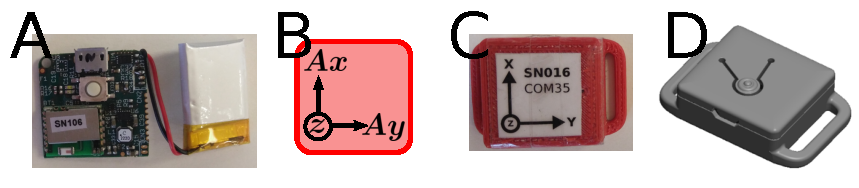
\includegraphics[width=1.0\textwidth]{muse}
   \caption{Inertial Measurament Sensor:
		(A) Printed Circuit Board (PCB) with 165mAh battery,
		(B) axis orientation, 
		(C) real case, and 
		(D) 3D model for the case.
}
   \label{fig:muse}
\end{figure}
%%---------------------------------(FIGURE)-------------------------------------

\section{Time-series preprocessing}
\subsection{Organising Data in Multidimensional Arrays}

Scripts in \MATLAB were created to syncronise the data using the clock drift and clock
offset values which were provided for each of the NeMEMSi sensors.
Then the data from each sensor is aligned in time using using
\texttt{finddelay()} and \texttt{alignsignals()} in \MATLAB.

The use of \texttt{alignsignals()} is useful when the data is relatively clean
that means that when data was noisy the alignment were not even close
when two signals were quite similar. Therefore, I decided to
program my own \texttt{alignsignalsMX()} to use the synchronised
data but with different length.


Scripts in \R  were used for postprocessing the data.

\subsection{Data Synchornisation}

To find the delay between two two sensors that were attached to the same place
of the body parts, a function called  \texttt{finddelayMX()} was created.
Such function computes the autocorrelation between two signals using \texttt(xcorr())
then the maximum value of the the autocorrleation function is extracted
to create a delay between the values of maximum index in the autocorrelation
function and the length of the first signal

% [R, lag] = xcorr(X,Y);
% [Y,I] = max(R);  %%%[Y,I] = max(X) returns the indices of the maximum values in vector I.
% delay = abs(I - length( X ) );

The function \texttt{alignsignalsMX()} was used to align two signals based
on \texttt{finddelayMX()}. The function \texttt{alignsignalsMX()} use six inputs
of which sA and sB are the sensors, then the windowframe of which the information
of the signal is extracted from another activities, the MainAxis of which the
signal are going to be extracted, the truncate delay that is created to
syncrohnise the signals adding an extra delay that is based on the lenght of
previous signals and tunning delay that can be useful to tune the delay in the
case of the dalay is not appropriate when the signals are too noisy.
% function [a,b,delay] =
% alignsignalsMX(sA,sB,windowframe,MainAxis,truncate_delay, tuning_delay)

Then, it is used the \texttt{aligntwosignals()} to align only two signals.
The inputs of \texttt{aligntwosignals()} are X and Y for the input vectors,
truncate delay for the previous delay of two signals and tunning delay
in case that signals are two noise and the xcorr fail to find an appropriate
delay.
 % function [a,b,delay] = aligntwosignals(X,Y,truncate_delay, tuning_delay)

\subsection{Time Alignment}
It was taken another approach to align the data in time in which the
original synchronised data is manipulated. Given four vectors of time
$t_1, t_2, t_3, t_4$, it is extracted the minimum and maximum values
of the start of the four sequence of time,
it was also exrtacted the minimum and maximum values to the
end of the four sequence of time.

However, after aligning the vectors it has then  been noticed that there were
different values of lenght across vectors i.e.: $1880,1986,1987,1988$
Therefore the lenght for the second vector was used as the primary lenght
becase is the one that is present the minimum value of the three maximum
lenghts. Then \texttt{interp1(x,v,vq,'phchip')}  was used to interpolate the
length of each of the vectors such as the length of all vectors is: $1986,1986,1986,1986$.
It has been choosen the \texttt{phchip} since the interpolation present
values for each of the points which were different for the NA values
from what it has been got when using \texttt{linear}.

\subsection{Issues with IMUs} \label{appendix:imus:issues}


\section{Humanoid robot}  \label{appendix:nao}
\subsection{Hardware}
\subsection{Software}




%!TEX root = ../thesis.tex
% ******************************* Thesis Appendix B ********************************

\chapter{Installing the CUED class file}

\LaTeX .cls  files can be accessed system-wide when they are placed in the
<texmf>/ tex/ latex directory, where <texmf> is the root directory of the user’s
\TeX installation.
On systems that have a local texmf tree (<texmflocal>), which
may be named ``texmf-local'' or ``localtexmf'', it may be advisable to install
packages in <texmflocal>, rather than <texmf> as the contents of the former,
unlike that of the latter, are preserved after the \LaTeX system is reinstalled
and/or upgraded.


\end{appendices}

% *************************************** Index ********************************
\printthesisindex % If index is present

\end{document}
